Environment reconstruction is an active field of research, it has been studied by the computer vision, photogrammetry and robotics communities. A particularly successful approach to this problem is known as Simultaneous Localization and Mapping (SLAM). The task in SLAM is to estimate the position of an entity (robot, car, person) by the metrics provided by sensors and at the same time construct a map of the environment~\cite{Thrun2008_SLAM}.

\begin{figure}[hb]
  \begin{center}
    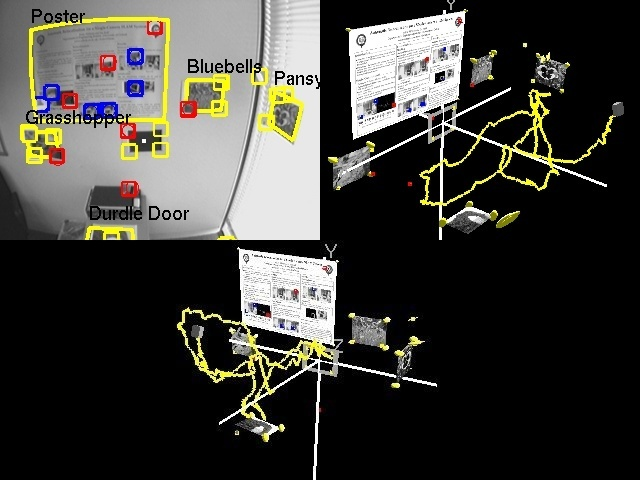
\includegraphics[width=0.5\textwidth]{slam-illustration-castle_etal_icra2007}
    \caption{The SLAM problem. From a series of sensed images (upper left corner), estimate the camera position (yellow lines) and recreate the scene (objects ``floating'')~\cite{slam-oxford-images}.}
  \end{center}
\end{figure}

%GPS unreliable because it's not precise, a couple of meters of difference could lead a car jumping on the curve or bumping another while trying to park.
Most research has cameras and/or a mixture of exotic depth sensors as inputs.
Depth sensors such as laser range finders are expensive, do not provide texture information and are bulky. That restricts mobile applications to vehicles where the cost of carrying such equipment is negligible (e.g. cars).
One variant of SLAM is to restrict the sensors to the visual type, this has been labelled as $visual$SLAM~\cite{Fuentes-Pacheco2012-slam}. Using cameras reduces the economical cost, but they still stream large quantities of information which has to be processed. If a real-time solution is desired, the most probable scenario is to run the algorithms in power-hungry devices. This is something that limits the actual utility for mobile systems with limited power resources. 
%Another disadvantage to using ``classic'' computer vision approaches is that computational resources would need to be shared inefficiently (i.e. a processor would have to switch between a facial recognition algorithm to a depth-estimation one). Having a neuro inspired system means that the tasks are executed by the same network.

Given that humans are able to do something similar with our brains, an efficient highly-parallel biological computing system that requires about 20-watts to function, we propose that a neural approach to SLAM is an energy-efficient way of solving the problem. The question of how exactly this is done in the brain is still open and is subject to research~\cite{rat-slam}. This work will provide a solution, inspired by state-of-the-art neuroscience, to the environment reconstruction problem using neuromorphic hardware.

If one is to develop a neural network based solution and remain power efficient, the only way to achieve this is on a neuromorphic processing platform. SpiNNaker provides a massively-parallel high-efficiency computing platform, inspired by the brain. These characteristics make it an excellent choice for neuroscience research, particularly to study spiking neural networks~\cite{furber2014spinnaker}. Furthermore, neuromorphic visual sensors have shown to reduce representations so that irrelevant information is not transmitted nor processed, though they are still in development and may be expensive~\cite{aer-retina-bernabe,dvs-zurich}. A combination of neuromorphic hardware and software will be the development platform for this project.
